\documentclass[a4paper,12pt]{article}
\usepackage[utf8x]{inputenc}
\usepackage[T2A]{fontenc}
\usepackage[russian,english]{babel}
\usepackage{amsmath}
\usepackage{cmap}
\usepackage{booktabs}
\usepackage{caption}
\usepackage{enumitem}
\usepackage{listings}
\usepackage{xcolor}
\usepackage{setspace}
\usepackage{graphicx}
\usepackage[left=2cm, right=1.5cm, top=2cm, bottom=2cm]{geometry}
\renewcommand{\labelenumii}{\arabic{enumi}.\arabic{enumii}.}
\lstset{
    language=C++,
    basicstyle=\small\ttfamily,
    keywordstyle=\color{blue},
    commentstyle=\color{green!40!black},
    stringstyle=\color{purple},
    numbers=left,
    numberstyle=\tiny,
    numbersep=5pt,
    breaklines=true,
    frame=single,
    backgroundcolor=\color{gray!10},
    rulecolor=\color{black!30},
    showstringspaces=false,
    extendedchars=\true, % Включение расширенных символов, включая русский текст
}

\begin{document}
	\renewcommand\contentsname{Содержание}
	\renewcommand{\arraystretch}{1.3} 
	\thispagestyle{empty}
	\begin{center}
		Министерство науки и высшего образования Российской Федерации\\
        Федеральное государственное автономное образовательное\\
        учреждение высшего образования
		\vspace{0.1cm}
		
		«Казанский (Приволжский)  Федеральный университет
		\vspace{1cm}
		
		ИНСТИТУТ ВЫЧИСЛИТЕЛЬНОЙ МАТЕМАТИКИ И ИНФОРМАЦИОННЫХ ТЕХНОЛОГИЙ
		
		Кафедра прикладной математики и искусственного интеллекта

		\vspace{1cm}

		Направление подготовки: 01.03.04 - «Прикладная математика»
	\end{center}
	\vspace{1cm}
	
	\begin{center}
		КУРСОВАЯ РАБОТА
		\vspace{0.2cm}
		
		по дисциплине: «Численные методы»
		\vspace{0.2cm}
		
		\textbf{Ограниченная задача трех тел.}
	\end{center}
	\vspace{3cm}
	Студент 2 курса\\
	группы 09-222\\
	«\underline{\qquad}» \underline{\qquad\qquad} 2024 г. \qquad\qquad\quad \underline{\qquad\qquad\qquad\quad} \qquad И.И. 	Романов\\
	Научный руководитель\\
	ассистент б. с.\\
	«\underline{\qquad}» \underline{\qquad\qquad} 2024 г. \qquad\qquad\quad \underline{\qquad\qquad\qquad\quad} \qquad О.В. 	Глазырина
	\vfill
	
	\begin{center}
		Казань, 2024
	\end{center}
	\newpage
	\begin{center}
		\renewcommand{\contentsname}{Содержание}
		\fontsize{14}{1.15}\selectfont
		\mdseries\selectfont{\tableofcontents}
		\newpage
	\end{center}
	\setlength{\parindent}{1.25cm}
	\newpage
	\selectfont\onehalfspacing{
	\begin{center}
		\section*{Постановка задачи}
		\addcontentsline{toc}{section}{1 Постановка задачи}
	\end{center}

    \par Рассмотрим два тела с массами $m$ (Луна) и $M=1-m$ (Земля), участвующие в совместном круговом движении в плоскости $xOy$ и расположенные в точках с координатами $(1,0)$ и $(0,0)$ соответственно. Пусть далее близ этих тел в той же плоскости движется третье тело пренебрежимо малой массы и $(x(t),y(t))$ - его координаты в момент времени $t$. Траектория движения этого тела описывается уравнениями:


\begin{equation}
    \begin{aligned}
		x'' &= x + 2y' - \dfrac{M(x + m)}{R_1} - \frac{m(x - M)}{R_2}, \\
		y'' &= y - 2x' - M \dfrac{y}{R_1} - m \frac{y}{R_2}, \\
		R_1 &= \left( (x + m)^2 + y^2 \right)^{3/2}, R_2 = \left( (x - M)^2 + y^2 \right)^{3/2}.
    \end{aligned}
	\label{1}
\end{equation}

Уравнения (1) дополняются начальными условиями:
\begin{equation}
x(0) = 0.994, \: y(0) = 0, \: x'(0) = 0, \: y'(0) = -2.031732629557337.
\label{2}
\end{equation}

При начальных условиях (2) и $m=0.012277471$ орбита будет периодической с периодом обращения, равным $T = 11.124340337$ (такие орбиты называют "орбитами Аренсторфа").

Для решения полученной задачи свести её к задаче Коши для системы уравнений первого порядка вида

$$ 
y' = f(t,y), \: y(0)=y_0, \: y(t) \in R^n
$$

и использовать метод Рунге-Кутты 4-го порядка точности:

\begin{equation}
    \begin{aligned}
		&k_1 = f(t_n, y_n), \quad &k_2 = f\left(t_n + \dfrac{h}{2}, y_n + \dfrac{h k_1}{2}\right), \\
		&k_3 = f\left(t_n + \dfrac{h}{2}, y_n + \dfrac{h k_2}{2}\right), \quad &k_4 = f\left(t_n + h, y_n + h k_3\right), \\
		&y_{n+1} = y_n + h (k_1 + 2k_2 + 2k_3 + k_4)/6.
    \end{aligned}
	\label{3}
\end{equation}


Для проверки правильности работы программы решить тестовую задачу из двух уравнений

\begin{equation}
	\begin{aligned}
	y_1'& = -y_2 + y_1 (y_1^2 + y_2^2 - 1), \\
	y_2'& = y_1 + y_2 (y_1^2 + y_2^2 - 1)
	\end{aligned}
	\label{4}
\end{equation}

на отрезке $[0, 5]$ с точным решением

$$
y_1 = \dfrac{\cos(x)}{\sqrt{1 + e^{2x}}}, \quad y_2 = \dfrac{\sin(x)}{\sqrt{1 + e^{2x}}}.
$$

\clearpage

В ходе работы необходимо выполнить следующие действия:
	
\begin{enumerate}
\item Проверить правильность тестового решения.
\item Написать процедуру интегрирования задачи Коши для системы из $\mathrm{n}$ обыкновенных дифференциальных уравнений второго порядка по формулам (3) на произвольном отрезке $[a, b]$ c постоянным шагом $\mathrm{h}$.
\item Для тестовой задачи (4) построить графики зависимости максимальной погрешности решения е и $e / h^4$ от выбранного шага $h$.
\item Рассчитать орбиту Аренсторфа. Учесть, что решения бесконечно дифференцируемы всюду за исключением двух точке $(-m,0)$, $(M,0)$. Поэтому в окрестности начала и конца отрезка интегрирования необходимо выбирать существенно меньший шаг инте\-гри\-ро\-вания $h$, чем в другие моменты времени. Построить график орбиты в координатах $(x,y)$
\end{enumerate}

\newpage
\begin{center}
	\section*{Ход работы}
	\addcontentsline{toc}{section}{3 Ход работы}
\end{center}
\par Для проверки тестовой задачи реализуем метод решения системы уравнений \eqref{4} с помощью формул \eqref{3}.
Так как система \eqref{4} является системой дифференциальных уравнений первого порядка, то никаких дополнительных замен переменных не потребуется.

В качестве начальных значений для нашей системы возьмём значения точных решений в начале отрезка $[0, 5]$ -- точке $0$. Откуда получим, что
\begin{equation*}
	y_1(0) = \frac{1}{\sqrt{2}}, \quad y_2(0) = 0.
\end{equation*}
Далее, выбрав значение шага $h = 0,01$, решим систему \eqref{4} методом Рунге-Кутты 4 порядка точности на отрезке $[0, 5]$ и сравним с точными решением системы. Получим данные графики:
\begin{figure}[ht]
	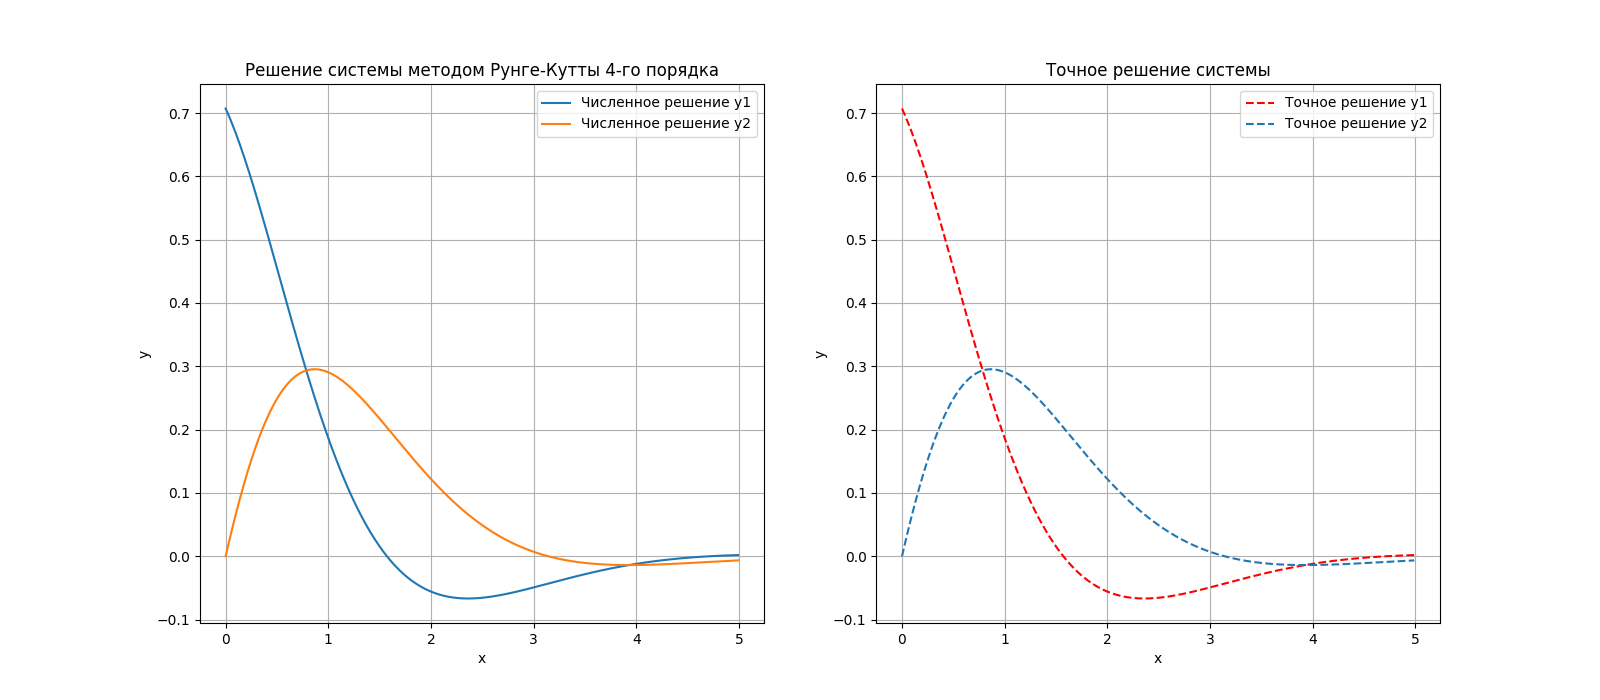
\includegraphics[width=\textwidth]{plot_test_task_exact_and_method.png}
	\caption*{{\small Рис.1 -- графики решения тестовой задачи методом Рунге-Кутты и точного решения}}
\end{figure}

Наложив данные графики друг на друга, убедимся, что решения сходятся:
\begin{figure}[ht]
	\centering
	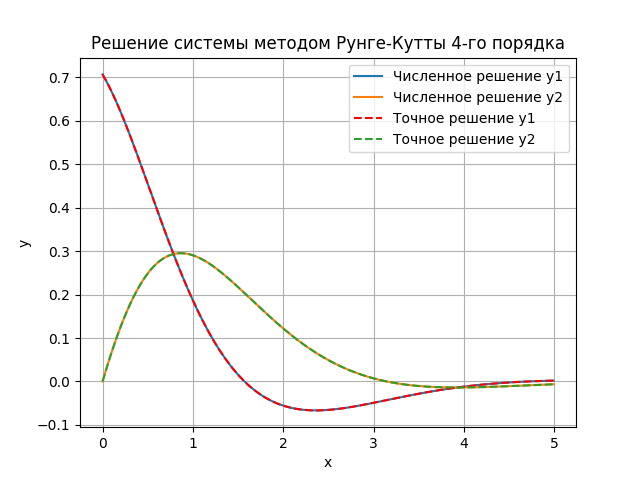
\includegraphics[width=7cm]{plot_test_task.png}
	\caption*{{\small Рис.2 -- наложенные графики решения методом Рунге-Кутты и точного решения}}
\end{figure}

Убедившись в правильности решения метода Рунге-Кутты 4 порядка точности, реали\-зуем процедуру интегрирования задачи Коши для системы из $n$\
уравнений второго порядка на произвольном отрезке $[a,b]$ с постоянным шагом $h$.

Пусть дана система обыкновенных дифференциальных уравнений второго порядка вида:
\begin{equation*}
	\begin{aligned}
		\frac{{d^2 y_1}}{{dt^2}} &= F_1(t, y_1, y'_1, y_2, y'_2, \ldots, y_n, y'_n) \\
		\frac{{d^2 y_2}}{{dt^2}} &= F_2(t, y_1, y'_1, y_2, y'_2, \ldots, y_n, y'_n) \\
		&\vdots \\
		\frac{{d^2 y_n}}{{dt^2}} &= F_n(t, y_1, y'_1, y_2, y'_2, \ldots, y_n, y'_n)
	\end{aligned}
\end{equation*}
где $y_i' = \dfrac{dy_i}{dt}$.

Данную систему можно преобразовать в эквивалентную систему из $2n$ обыкновенных дифференциальных уравнений первого порядка, сделав замену переменных.
Введём новые переменные $z_i = \dfrac{dy_i}{dt}$, чтобы сделать эквивалентное преобразование. Получим систему вида:
\begin{equation*}
	\begin{aligned}
		\frac{{dy_1}}{{dt}} &= z_1 \\
		\frac{{dz_1}}{{dt}} &= F_1(t, y_1, z_1, y_2, z_2, \ldots, y_n, z_n) \\
		\frac{{dy_2}}{{dt}} &= z_2 \\
		\frac{{dz_2}}{{dt}} &= F_2(t, y_1, z_1, y_2, z_2, \ldots, y_n, z_n) \\
		&\vdots \\
		\frac{{dy_n}}{{dt}} &= z_n \\
		\frac{{dz_n}}{{dt}} &= F_n(t, y_1, z_1, y_2, z_2, \ldots, y_n, z_n)
	\end{aligned}
\end{equation*}

Получив систему из $2n$ обыкновенных дифференциальных уравнений первого порядка, при\-ме\-ним начальные значения системы второго порядка для получившейся системы.
Далле для каждого получившегося уравнения системы обыкновенных дифференциальных уравне\-ний первого порядка применим метод Рунге-Кутты 4 порядка точности на отрезке $[a,b]$ с точным шагом $h$.

Правильность решения метода Рунге-Кутты 4 порядка точности во многом зависит от выбранного значения $h$. На примере тестовой задачи рассмотрим поведение максимальной ошибки вычисления в зависимоти от выбранного значения $h$.
Для этого проведём вычисления тестовой задачи для $h = 0,001,\;\dots,\;0,1$, постепенно увеличивая шаг. Рассмотрим значение максимальной ошибки вычисления $e$ и $e/h^4$ для данных шагов.

Построим графики зависимостей:
\begin{figure}[ht]
	\centering
	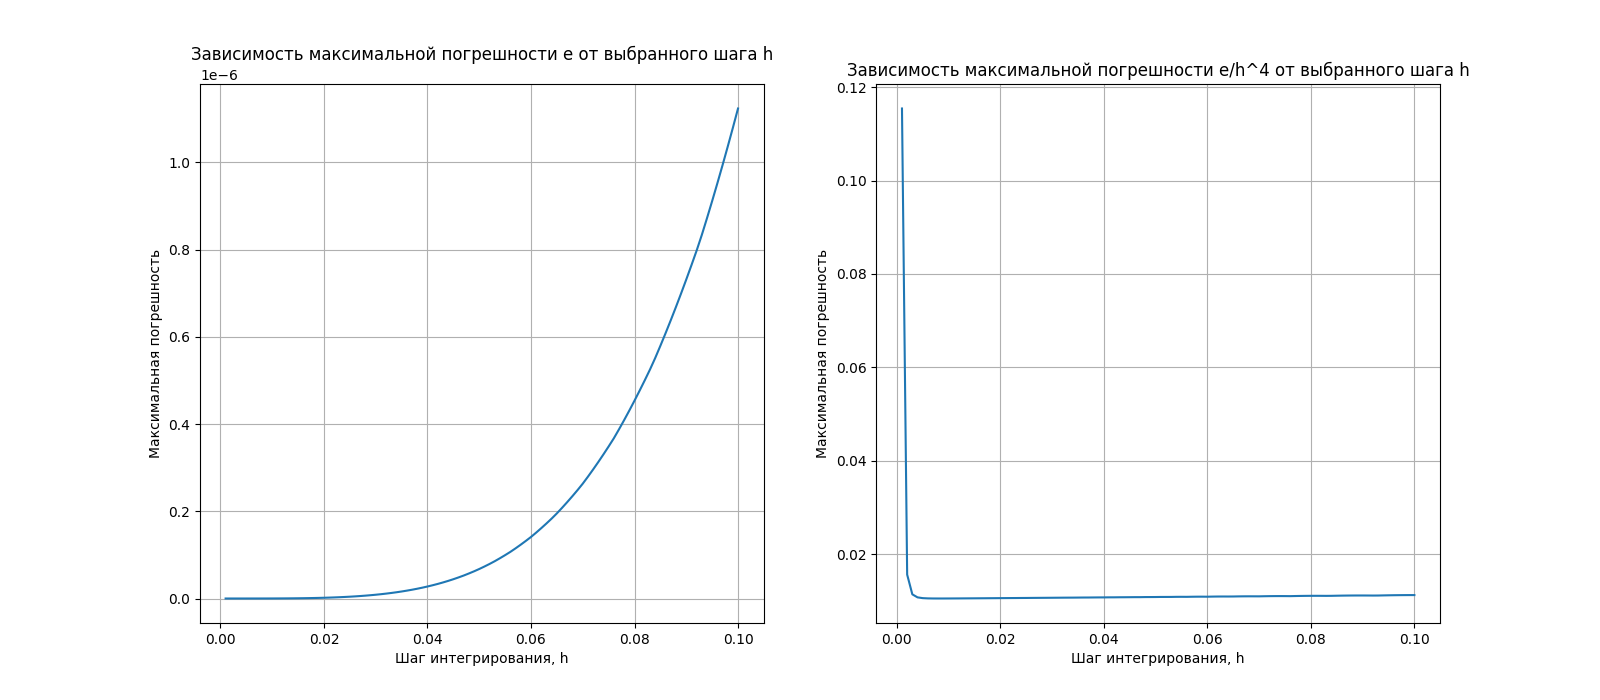
\includegraphics[width=\textwidth]{plot_max_err.png}
	\caption*{{\small Рис.3 -- графики зависимости значения максимальной ошибки $e$ и $e/h^4$ от выбранного шага $h$}}
\end{figure}
Данные графики показывают, что значение макси\-мальной вычислительной ошибки $e$ возрастают с уравнением значения шага $h$.

Теперь расчитаем орбиту Аренсторфа, решив систему \eqref{1} с начальными условиями \eqref{2} при помощи формул \eqref{3} метода Рунге-Кутты 4 порядка точности.
Пусть \( u_1 = x \), \( u_2 = x' \), \( u_3 = y \), и \( u_4 = y' \).

Мы можем записать систему \eqref{1} с помощью обыкновенных дифференциальных урав\-не\-ний первого порядка в следующем виде:

\begin{equation}
	\begin{cases}
	u'_1 = u_2 \\
	u'_2 = u_1 + 2u_4 - M\frac{(u_1 - m)}{R_1^{\frac{3}{2}}} - m\frac{(u_1 - M)}{R_2^{\frac{3}{2}}} \\
	u'_3 = u_4 \\
	u'_4 = u_3 - 2u_2 - M\frac{u_3}{R_1^{\frac{3}{2}}} - m\frac{u_3}{R_2^{\frac{3}{2}}}
	\end{cases}
	\label{5}
\end{equation}

Теперь определим \( R_1 \) и \( R_2 \):

\[
R_1 = \left((u_1 + m)^2 + u_3^2\right)^{\frac{3}{2}}, \quad R_2 = \left((u_1 - M)^2 + u_3^2\right)^{\frac{3}{2}}
\]

Определим начальные условия:
\begin{equation*}
	u_1(0) = 0,994,\;u_2(0) = 0,\;u-3(0) = 0,\;u_4(0) = -2,031732629557337
\end{equation*}

Далее определимся с отрезком интегрирования. Поскольку нужная нам орбита Арен\-сторфа имеет период обращения $T = 11.124340337$, то будем считать,
что отрезком инте\-гри\-рования будет служить $[0,T]$. Шаг возьмём равным $h = 0.01$.

Определившись с отрезком интегрирования и шагом, реализуем метод Рунге-Кутты 4 порядка точности по формулам \eqref{3} для получившейся системы \eqref{5}.

Вычисления строим таким образом, чтобы учесть тот факт, что решения задачи бесконечно дифференцируемы всюду, кроме точек $(-m, 0)$ $(M, 0)$.
В окрестности начала и конца отрезка интегрирования выберем существенно меньший шаг интегрирования $h$. Построим график орбиты Аренсторфа.
\begin{figure}[ht]
	\centering
	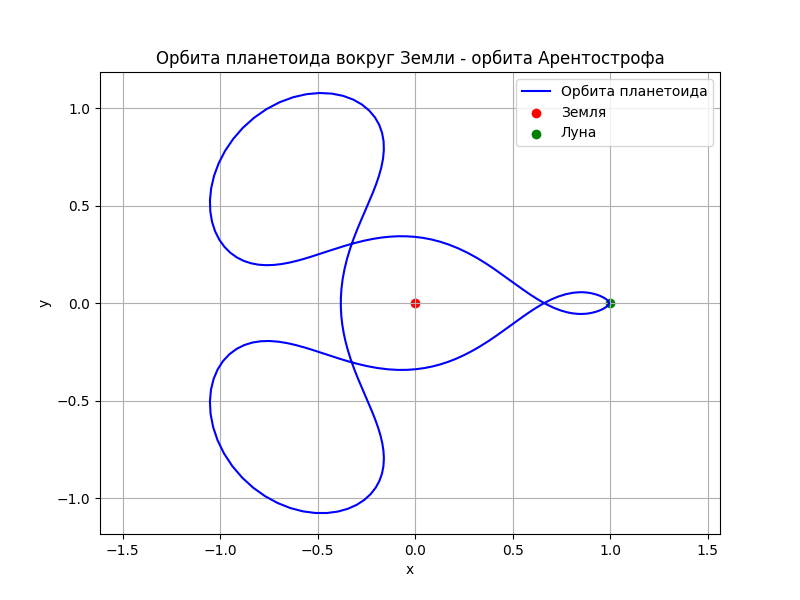
\includegraphics[width=\textwidth]{plot_main_task.png}
	\caption*{{\small Рис.4 -- график орбиты Аренсторфа}}
\end{figure}

График описывает орбиту планетоида, который движется под влиянием гравитации Земли и Луны.
Синяя линия показывает траекторию движения планетоида. Орбита имеет сложную форму и включает в себя несколько замкнутых петель.
Данная орбита харак\-те\-ризуются тем, что планетоид периодически приближается и удаляется от Земли и Луны.

На графике видно три основные петли орбиты планетоида: две крупные петли выше и ниже оси x, и одна маленькая петля справа от Земли и Луны.
Петли показывают, что планетоид проходит близко к Земле и Луне, а затем удаляется от них на большие расстояния.
Когда планетоид находится на петлях, он испытывает сильное гравитационное влияние как Земли, так и Луны.

Движение планетоида описывается периодическим характером: он возвращается в определенные точки своей орбиты спустя фиксированные промежутки времени.
Орбита не является стабильной и регулярной.
\clearpage
\begin{center}
	\section*{Вывод}
	\addcontentsline{toc}{section}{4 Вывод}
\end{center}
\par В ходе выполнении курсовой работы, была решена тестовая задача и реализована программа интегрирования задачи Коши с 
помощью Рунге- Кутты 4-го порядка точности с постоянным шагом h для системы, состоящей из $n$ обыкновенных дифференциальных уравнений. Были построены графики зависимости максимальной 
погрешности решения $e$ и $e/h^4$ от выбранного шага h. По графикам можно сделать вывод, что максимальная погрешность
решения e возрастает при увеличении шага h. Был построен график орбиты Аренсторфа.
\newpage
\begin{center}
	\section*{Список литературы}
	\addcontentsline{toc}{section}{5 Список литературы}
\end{center}
\begin{enumerate}
	\item Даутов Р. З. Практикум по дисциплине “Численные методы”. Решение задачи Коши для системы ОДУ. - Учебное пособие, Казань, 2014.
	\item Хайрер Э., Нерсетт С., Ваннер Г. Решение обыкновенных дифференциальных уравнений. - М.: Мир, 1990.
	\item Самарский А.А., Гулин А.В. Численные методы. - М.: Наука, 1989.
	\item Бахвалов Н.С., Жидков Н.П., Кобельков Г.М. Численные методы. - М.: Наука, 1987.
  \end{enumerate}

\newpage
}
\begin{center}
	\section*{Листинг}
	\addcontentsline{toc}{section}{6 Листинг}
\end{center}
\lstinputlisting[language=Python]{./test_task.py}
\lstinputlisting[language=Python]{./task2.py}
\lstinputlisting[language=Python]{./task_main.py}
\end{document}